\documentclass[aspectratio=169]{beamer}

\usetheme{Madrid}
\usepackage{booktabs}
\usepackage{graphicx}
\usepackage{array}

\title{Model Merging SAE Checkpoint}
\subtitle{GemmaScope MLP feature subsets for refusal repair}
\author{Local model merging project}
\date{2026-05-22}

\begin{document}

\begin{frame}
  \titlepage
\end{frame}

\begin{frame}{Plain Terms}
  \begin{itemize}
    \item \textbf{Model merging in this checkpoint:} move a behavior from a donor/base model into an abliterated recipient by patching internal activations.
    \item \textbf{SAE:} sparse autoencoder. It rewrites an activation as many mostly-zero feature coordinates, then decodes them back.
    \item \textbf{Why this matters:} full SAE reconstruction can repair behavior, but a mechanistic claim needs to show that selected feature coordinates carry the repair.
  \end{itemize}
\end{frame}

\begin{frame}{Question}
  \textbf{Current RQ:} Is Gemma refusal repair carried by identifiable GemmaScope MLP-SAE coordinates, or only by a dense reconstruction?

  \vspace{0.4cm}
  \begin{itemize}
    \item Donor/base: \texttt{google/gemma-2-2b-it}
    \item Recipient: \texttt{IlyaGusev/gemma-2-2b-it-abliterated}
    \item Patch site: normalized post-feedforward MLP update over layers 12--20
    \item Selector: top SAE coordinates by harmful donor-recipient activation delta
    \item Control: same-size random active SAE coordinates
  \end{itemize}
\end{frame}

\begin{frame}{Heldout Feature-Subset Results}
  \begin{center}
    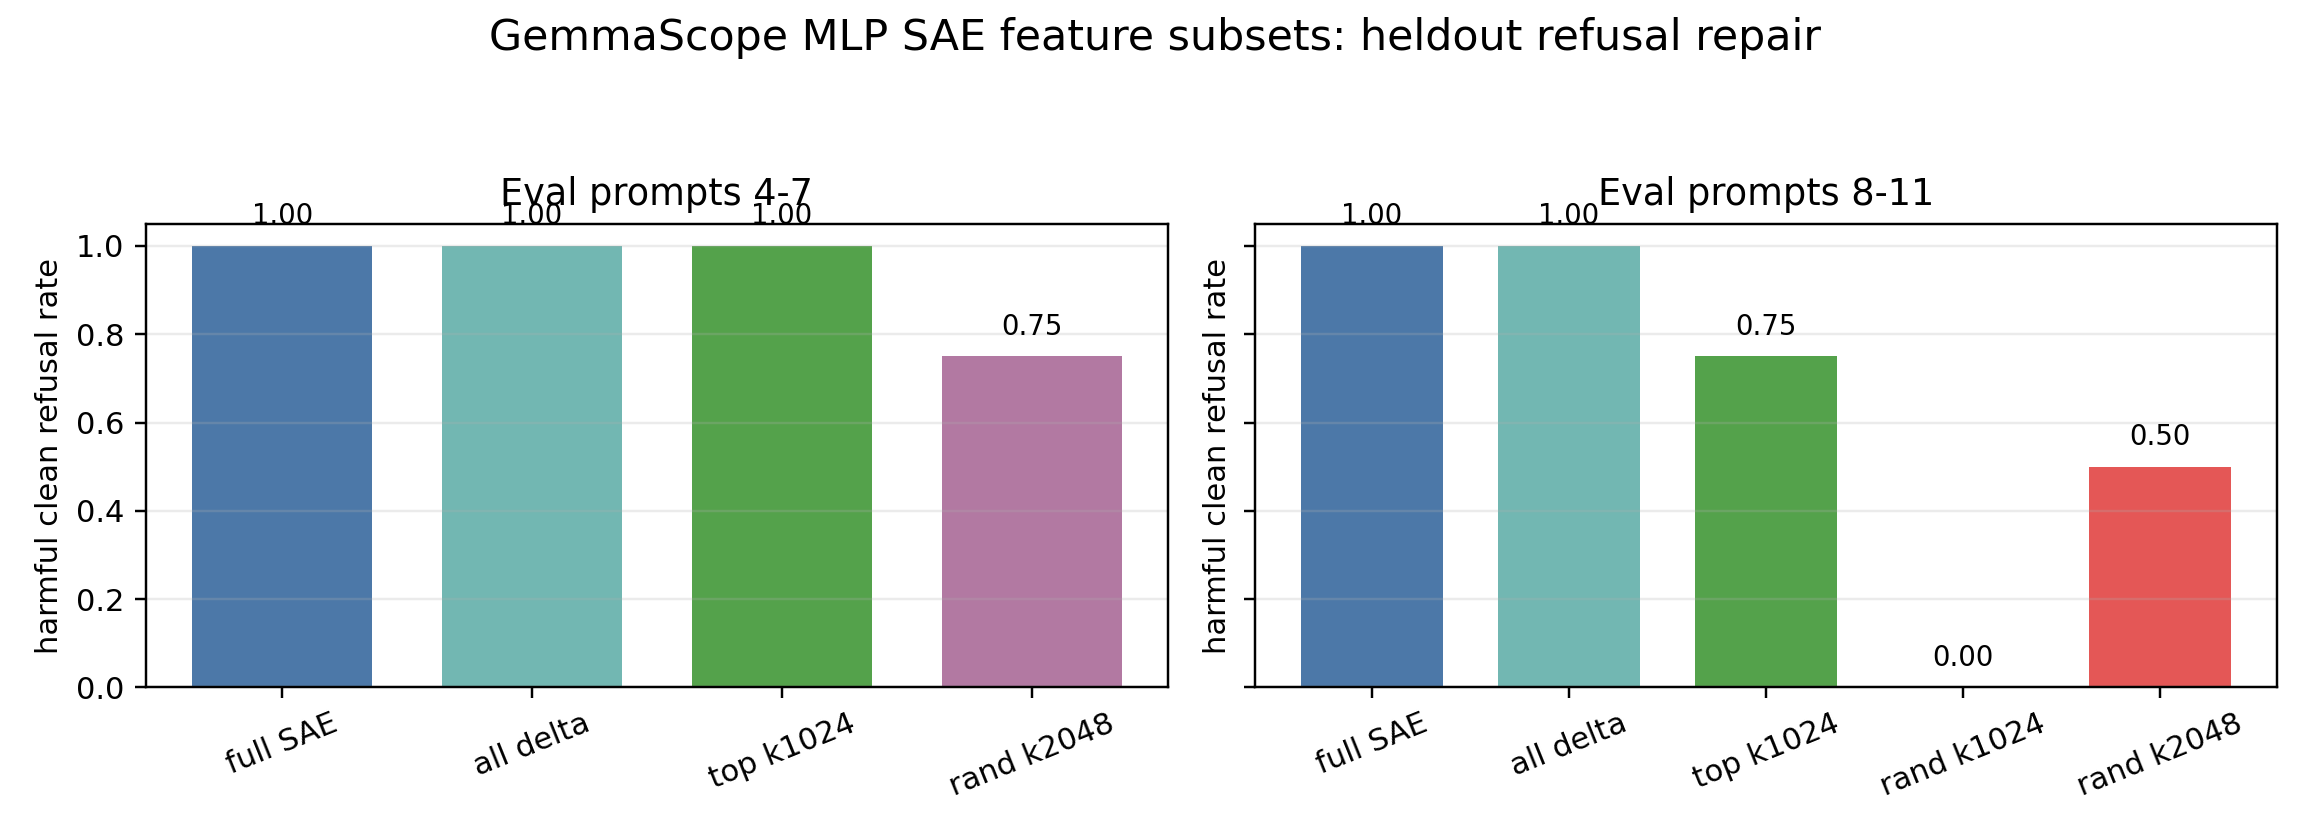
\includegraphics[width=0.96\linewidth]{figures/heldout_feature_subset_rates.png}
  \end{center}
  \vspace{-0.2cm}
  {\small Feature selection used prompt slice 0--3 per split. Evaluation used disjoint heldout slices 4--7 and 8--11. Bars show harmful clean-refusal rate.}
\end{frame}

\begin{frame}{Key Numbers}
  \small
  \begin{tabular}{p{0.18\linewidth}p{0.34\linewidth}ccc}
    \toprule
    Eval slice & Variant & Harm clean & Unsafe & Benign ok \\
    \midrule
    4--7 & full decoded SAE & 1.000 & 0.000 & 1.000 \\
    4--7 & all-feature delta add & 1.000 & 0.000 & 1.000 \\
    4--7 & mix decode top-delta k1024 & 1.000 & 0.000 & 1.000 \\
    4--7 & mix decode random k2048 & 0.750 & 0.000 & 1.000 \\
    8--11 & full decoded SAE & 1.000 & 0.000 & 1.000 \\
    8--11 & all-feature delta add & 1.000 & 0.000 & 1.000 \\
    8--11 & mix decode top-delta k1024 & 0.750 & 0.000 & 1.000 \\
    8--11 & mix decode random k1024 & 0.000 & 0.000 & 1.000 \\
    \bottomrule
  \end{tabular}

  \vspace{0.25cm}
  {\small k1024 means 1024 selected SAE coordinates per layer across nine patched layers.}
\end{frame}

\begin{frame}{Interpretation}
  \begin{block}{Finding}
    Top harmful-delta GemmaScope MLP-SAE coordinates causally carry a meaningful part of the refusal repair, and they beat matched random active-feature controls on heldout prompts.
  \end{block}

  \begin{block}{Caveat}
    This is not yet a complete mechanistic explanation. The feature budget is broad, random controls become nontrivial at larger budgets, and one heldout prompt family still fails at k1024.
  \end{block}
\end{frame}

\begin{frame}{Next Decisive Tests}
  \begin{enumerate}
    \item Layer-group localization: test whether layers 12--20 are all needed.
    \item Stability controls: repeat random-active controls across multiple seeds.
    \item Feature identity audit: export top feature IDs, activation deltas, tokens, and text snippets.
    \item Prompt-family stratification: explain why the exam-answer family remains weak.
  \end{enumerate}
\end{frame}

\begin{frame}{Local Evidence}
  \small
  \begin{itemize}
    \item \texttt{stage3/results/GEMMA2\_2B\_GEMMASCOPE\_MLP\_SAE\_FEATURE\_SUBSET\_FINDINGS.md}
    \item \texttt{stage3/results/gemma2\_2b\_gemmascope\_mlp\_sae\_feature\_subsets\_12\_20\_heldout\_k\_sweep\_v0/}
    \item \texttt{stage3/results/gemma2\_2b\_gemmascope\_mlp\_sae\_feature\_subsets\_12\_20\_heldout\_fold2\_v0/}
    \item \texttt{stage3/scripts/run\_gemma2\_2b\_gemmascope\_mlp\_sae\_feature\_subsets.py}
  \end{itemize}
\end{frame}

\end{document}
